%  LaTeX support: latex@mdpi.com 
%  For support, please attach all files needed for compiling as well as the log file, and specify your operating system, LaTeX version, and LaTeX editor.

%=================================================================
\documentclass[gene,journal,article,submit,moreauthors,pdftex]{Definitions/mdpi} 
\usepackage{natbib}
\usepackage[colorinlistoftodos]{todonotes}
%\usepackage[dvipsnames]{xcolor}
\newcounter{mycomment}
\newcommand{\mycomment}[2][]{%
% initials of the author (optional) + note in the margin
\refstepcounter{mycomment}%
{%
\setstretch{0.7}% spacing
\todo[color={red!100!green!33},size=\small]{%
\textbf{Comment [\uppercase{#1}\themycomment]:}~#2}%
}}
% For posting an early version of this manuscript as a preprint, you may use "preprints" as the journal and change "submit" to "accept". The document class line would be, e.g., \documentclass[preprints,article,accept,moreauthors,pdftex]{mdpi}. This is especially recommended for submission to arXiv, where line numbers should be removed before posting. For preprints.org, the editorial staff will make this change immediately prior to posting.

%--------------------
% Class Options:
%--------------------
%----------
% journal
%----------

%---------
% article
%---------
% The default type of manuscript is "article", but can be replaced by: 
% abstract, addendum, article, book, bookreview, briefreport, casereport, comment, commentary, communication, conferenceproceedings, correction, conferencereport, entry, expressionofconcern, extendedabstract, datadescriptor, editorial, essay, erratum, hypothesis, interestingimage, obituary, opinion, projectreport, reply, retraction, review, perspective, protocol, shortnote, studyprotocol, systematicreview, supfile, technicalnote, viewpoint, guidelines, registeredreport, tutorial
% supfile = supplementary materials

%----------
% submit
%----------
% The class option "submit" will be changed to "accept" by the Editorial Office when the paper is accepted. This will only make changes to the frontpage (e.g., the logo of the journal will get visible), the headings, and the copyright information. Also, line numbering will be removed. Journal info and pagination for accepted papers will also be assigned by the Editorial Office.

%------------------
% moreauthors
%------------------
% If there is only one author the class option oneauthor should be used. Otherwise use the class option moreauthors.

%---------
% pdftex
%---------
% The option pdftex is for use with pdfLaTeX. If eps figures are used, remove the option pdftex and use LaTeX and dvi2pdf.
%=================================================================
% MDPI internal commands
\firstpage{1} 
\makeatletter 
\setcounter{page}{\@firstpage} 
\makeatother
\pubvolume{1}
\issuenum{1}
\articlenumber{0}
\pubyear{2021}
\copyrightyear{2020}
%\externaleditor{Academic Editor: Firstname Lastname} % For journal Automation, please change Academic Editor to "Communicated by"
\datereceived{} 
\dateaccepted{} 
\datepublished{} 
\hreflink{https://doi.org/} % If needed use \linebreak
%------------------------------------------------------------------
% The following line should be uncommented if the LaTeX file is uploaded to arXiv.org
%\pdfoutput=1

%=================================================================
% Add packages and commands here. The following packages are loaded in our class file: fontenc, inputenc, calc, indentfirst, fancyhdr, graphicx, epstopdf, lastpage, ifthen, lineno, float, amsmath, setspace, enumitem, mathpazo, booktabs, titlesec, etoolbox, tabto, xcolor, soul, multirow, microtype, tikz, totcount, changepage, paracol, attrib, upgreek, cleveref, amsthm, hyphenat, natbib, hyperref, footmisc, url, geometry, newfloat, caption
\usepackage{hyperref}
\usepackage[utf8]{inputenc}
\usepackage[spanish,english]{babel}
%=================================================================
%% Please use the following mathematics environments: Theorem, Lemma, Corollary, Proposition, characterisation, Property, Problem, Example, ExamplesandDefinitions, Hypothesis, Remark, Definition, Notation, Assumption
%% For proofs, please use the proof environment (the amsthm package is loaded by the MDPI class).

%=================================================================
% Full title of the paper (Capitalized)
\Title{A crop modelling strategy to improve cacao quality and productivity }

% MDPI internal command: Title for citation in the left column
\TitleCitation{Title}

% Author Orchid ID: enter ID or remove command
\newcommand{\orcidauthorA}{0000-0000-0000-000X} % Add \orcidA{} behind the author's name
%\newcommand{\orcidauthorB}{0000-0000-0000-000X} % Add \orcidB{} behind the author's name

% Authors, for the paper (add full first names)
\Author{Angela P. Romero V. $^{1,\ddagger}$*\orcidA{}, Anyela V. Camargo R.$^{1, \ddagger}$, Oscar D. Ramirez$^{3}$, Paula A. Arenas V$^{3}$ and Adriana M. Gallego$^{2}$}

% MDPI internal command: Authors, for metadata in PDF
\AuthorNames{Firstname Lastname, Firstname Lastname and Firstname Lastname}

% MDPI internal command: Authors, for citation in the left column
\AuthorCitation{Romero, A.P.V;  Camargo, A.; Arenas P.; Ramirez O. D.; Gallego, A.;}
% If this is a Chicago style journal: Lastname, Firstname, Firstname Lastname, and Firstname Lastname.

% Affiliations / Addresses (Add [1] after \address if there is only one affiliation.)
\address{$^{1}$ \quad The John Bingham Laboratory, NIAB, 93 Lawrence Weaver Road, Cambridge CB3 0LE, UK \\$^{2}$ \quad Grupo BIOS, Centro de Bioinformática y Biología Computacional de Colombia - BIOS, Manizales, Caldas, Colombia, South America.\\ $^{3}$ \quad Federación Nacional de Cafeteros FEDECACAO, Colombia, South America. }%; e-mail@e-mail.com}

% Contact information of the corresponding author
\corres{Correspondence: ing.aromerov@gmail.com; anyela.camargorodriguez@niab.com} %; Tel.: (optional; include country code; if there are multiple corresponding authors, add author initials) +xx-xxxx-xxx-xxxx (F.L.)}

% Current address and/or shared authorship
%\firstnote{Current address: Affiliation 3} 
\secondnote{These authors contributed equally to this work.}
% The commands \thirdnote{} till \eighthnote{} are available for further notes

%\simplesumm{} % Simple summary

%\conference{} % An extended version of a conference paper

% Abstract (Do not insert blank lines, i.e. \\) 


\abstract{Cacao production systems in Latin America have a high importance over social and economic development, facing  the fight against hunger and poverty. Although Colombian cacao has the potential to be in the high value markets for fine flavour, the lack of expert support as well as the use of traditional, and often times suboptimal, technologies makes cocoa production negligibly. \textcolor{blue}{Traditionally cacao harvest takes place at 5 or 6 months  by calendar after flowering, the problem is that  the seeds are often  unripe or  over ripe germinating inside the pod afecting the quality of the final cocoa products}. Other environmental parameters that have more association with pod maturation speed are not taken into account.  Cacao fruits development can be considered as the result of a number of physiological and morphological processes that can be described by mathematical relationships even under uncontrolled environments. In this context, crop models are useful tools to simulate and predict crop development over time and under multiple environmental conditions. Since, harvesting at the right time can yield high quality cacao, we parametrised a crop model to predict the best time for harvest cocoa fruits in Colombia. . Results can be a practical tool that supports cacao farmers in the production of high quality cocoa.  When comparing simulated and observed data, our results showed an RRMSE of 7.2\% for the yield prediction, while the simulated harvest date varied between +/- 2 to 20 days depending on the temperature variations of the year between regions. This crop model contributed to understand and predict the phenology of cacao fruits for two key cultivars ICS95 y CCN51. \textcolor{blue}{The aim of this study was to calibrate a crop model that simulates cacao crop development and yield, and predicts the maturation day when the fruit is likely to be ready for harvest which will improve the quality of the seeds.}}  

% Keywords
\keyword{thermal time, flowering date (FD), harvest prediction, biomass, light interception } 

%%%%%%%%%%%%%%%%%%%%%%%%%%%%%%%%%%%%%%%%%%
\begin{document}
%%%%%%%%%%%%%%%%%%%%%%%%%%%%%%%%%%%%%%%%%%
%\setcounter{section}{-1} %% Remove this when starting to work on the template.

\section{Introduction}

Cacao ( \textit{Theobroma cacao }L. ) is an important worldwide perennial tropical crop endemic to the South American rainforests \citep{zuidema2005, motamayor2002, argout2011, Rodriguez2019}. Cacao plant is a member of the Malvaceae (formerly Sterculiaceae)  botanical family such as  cotton \textit{ Gossypium hirstium} \citep{Nix2017cotton}. Cotton has been is modelled in SIMPLE model \citep{Zao2019simple}. Cacao is grown for its fruits, known as cacao pods \citep{ Niemenak2010, suarez2021}. Only the 5\% of the world cocoa yield is destined for Fine-cocoa production due to the low productivity through  the traditional crop management \citep{argout2011}.  In Colombia, cocoa  is  traditionally  consumed  as  a  beverage. It is one of the crops promoted by the Colombian government in the social and agricultural development  programs aimed at favouring peace in post-conflict regions \citep{Rodriguez2019, Abbott2019}. This crop is grown by approximately 52.000 families \citep{Gutierrez2020} and 98\% of production being carried out by small and medium-sized producers \citep{Garcia2014, Escobar2020}. Colombia registered an increase of 3.750 tons in production in 2020 compared to the previous year \citep{lamos2020}. 

Although Colombian cocoa has the potential to be in the high value markets for fine flavour \citep{Escobar2020}, the lack of expert support as well as the use of traditional, and often times suboptimal, technologies makes cocoa production negligibly. The farmer practice of empirically harvesting from 5 to 6 months or 180 Days After Flowering  (DAF) date, produced a mix of quality of cacao beans that are then fermented. \textcolor{blue}{The problem is that  the seeds are often  unripe or  over ripe germinating inside the pod affecting the cocoa quality}. This practice produces heterogeneous characteristics between each fermentation batch which potentially diminish the quality of the final cocoa product \citep{Escobar2021}.  \textcolor{blue}{Therefore,  It is important to identify the best moment to harvest  considering physiological responses affected by  soil types , cultivar specifications and weather variables such as rain, solar radiation and wind.  Thus,  for cacao production in Colombia, physiological simulation models may be valuable to predict the right moment to harvest cocoa fruits, hence it will improve the quality of seeds.}

Crop models represent a quantitative assumption of plant growth depending on sunlight interception efficiency values and climate data supported by a large amount of empirical and ground data. \citep{Reynolds2018}. Physiological crop models have shown to be very useful tool for provided agronomical advices and improvements of the cropping systems of annual crops mainly. Recently crop modelling studies are focusing on  perennial crops  production \citep{zuidema2005, Zao2019simple, Bai2020, Romero2021}. However, the information reported  is less than for annual crops due to the lack of field data available , relatively high research costs and the difficulties of accumulated errors in long-term simulations \citep{zuidema2005}. For cacao there are  approaches  to predict yield mainly  using algorithms of machine learning \citep{lamos2020} and just one mechanistic model simulates physiological cocoa performance  "SUCROS-cocoa" \citep{zuidema2005}. This crop model calculates light interception, photosynthesis, maintenance respiration,
evapotranspiration, biomass production and cocoa yield. It can be parametrised having data on cocoa physiology and morphology \citep{zuidema2005}. However,  there is not specific cocoa physiology data available from small and medium-sized producers. Thus, we adapted the simple generic crop model (SIMPLE) that could be easily modified for any crop to simulate development, crop growth and yield using few parameters such as weather and cultivar specification \citep{Zao2019simple}.

In this paper, we present a physiological parametrisation of the SIMPLE crop model \citep{Zao2019simple} for cocoa to predict best harvest time and overall yield in the framework of KOCOLATL project, which is a collaborative work between Colombian partners (researches, farmers and organizations such as Fedecacao and BIOS) and researchers in NIAB from United Kingdom. We parametrised this crop model  because it had already been successfully fitted to other tree crops in south America.  Our aim was to calibrate a crop model that simulates crop development, growth and yield, and predicts the maturation day when the fruit is likely to be ready for harvest. Results can be a practical tool that supports cacao farmers in the production of high quality cocoa. Thus, making Colombian cacao more competitive in the Fine-cocoa market.

\subsection{Floral Phenology of Cacao}

The phenological stages of a cacao tree are divided in two main phases, vegetative and reproductive. The reproductive phase (fig. \ref{fig:pheno}, a) is represented by the floral phenology which goes from the date of inflorescence emergence (BBCH scale 5) (fig. \ref{fig:pheno},b ) to the date of ripening of fruit and seed (BBCH 8) (fig. \ref{fig:pheno},c ) \citep{Niemenak2010}. The reproductive phase is cyclically across two annual cycles which go through the following phases: inflorescence emergence, flowering, pollination, fruit development and harvest. Therefore, to model the cacao crop cycle as perennial plant, we regarded the the start point of the cocoa crop cycle as the inflorescence emergence date, as opposed to the sowing/emergence date usually used to model annual crops (fig. \ref{fig:pheno},b). Therefore, the growth period of the fruit could vary from 110 to 150 daa (days after anthesis) \citep{lopez2018} when cacao fruits reach the physiological maturity, but it can be harvested at 170 days daa \citep{Niemenak2010} for quality purposes.

Since cacao is a cauliflorous plant, flowers grow on trunk and branches. Cacao trees usually produce up to 10000 flowers per tree each year, 50 \%  of which do not develop into ripe fruits (Personal communication with Fedecacao). Flower development takes approximately 30 days across 12 micro-stages, from meristem growth (stages 1 to 6) to the fully developed flower (Stages 7 to 12) \citep{swanson2005, lopez2018} when it is ready to be pollinated. The opening of flowers or anthesis  occurs over a 12-hour period during the night and it is synchronised between the groups of mature flowers \citep{Niemenak2010}. However, the life of a flower can last approximately 1 day after the opening, when it falls form the trunk if it is unfertilised \citep{cheesman1927, Niemenak2010}. Subsequentially, after anthesis, fruits growth for approximately 150 days until the maturation, mucilage. Therefore, the complete maturation process of the fruit, from the pollination to fully mature fruit, takes 160- 210 days \citep{berry1994}. The accumulation of lipids, storage proteins and anthocyanin start about 85 days after pollination when fruits have an active metabolism and seeds moisture content decreases up to 30\% \citep{Lehrian1980, Niemenak2010}. During this phase the quality of cocoa seeds is defined.


\begin{figure}[h!]
	\centering
	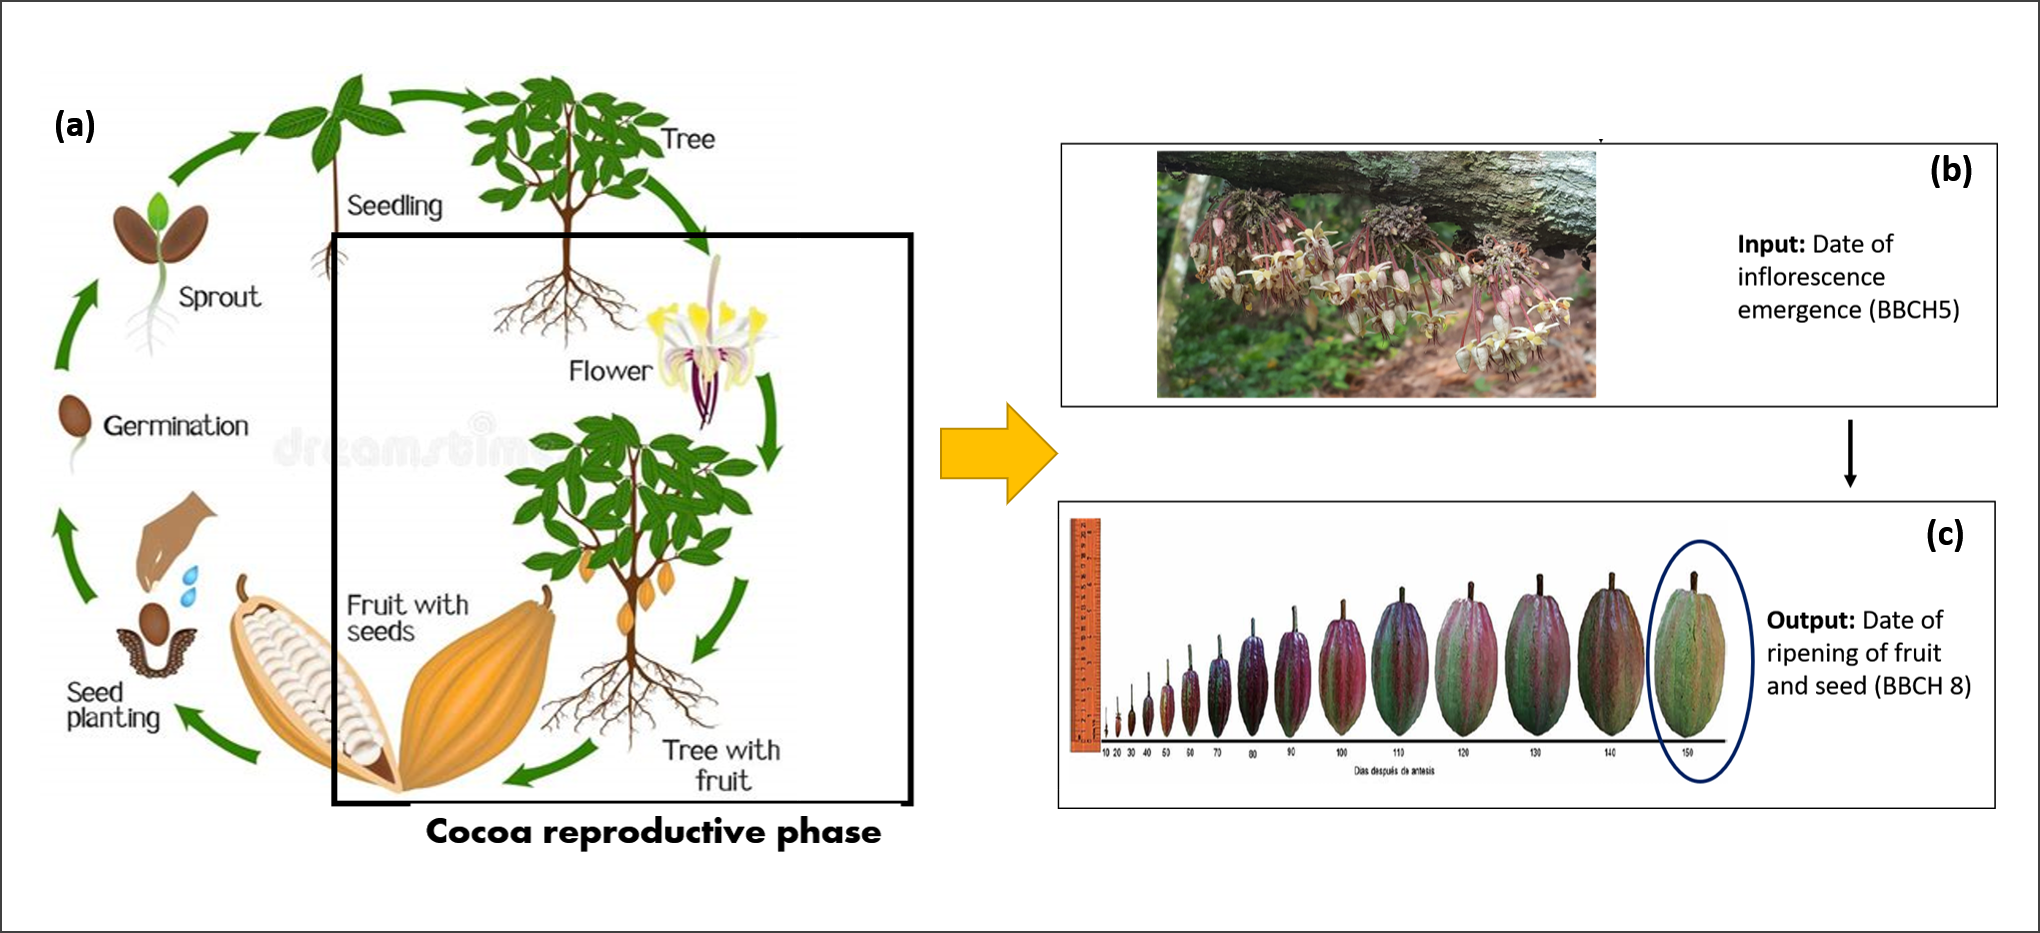
\includegraphics[scale=0.15]{images/phenology.png}\\
	\caption{\footnotesize {Phenology of cocoa in Colombia for crop modelling.\\}} 
	\footnotesize{Source: Taken from Dreamstime.com, phys.org \citep{toledo2021} and \cite{lopez2018}}
	\label{fig:pheno}
\end{figure}

\section{Materials and Methods}



\subsection{Test Site and Yield Production }

To calibrate and evaluate the cacao model, 23 field data samples were collected by Fedecacao, from five farms located in the geographic regions of Saravena (Arauca), Rionegro (Santander), Cali (Valle del Cauca), Apartado (Antioquia) and Manizalez (Caldas) (Fig.\ref{fig:yield}, a). Each field sample reported an observed flowering date and corresponding yield, for a given tree and month of the year. Field samples reported sights of 23 flowering dates from 12-July-2019 to 23-June-2020. Each of these dates had their corresponding date of harvest after at exactly 180 DAF,  the age of the trees, plant density (trees ha$^{-1}$), yield  (dry beans kg ha$^{-1}$) and number of fruits harvested per hectare. Thus, 23 flowering dates for five farms gave us 115 samples in total.

\subsection{Weather Conditions }
We analysed and compared weather patterns linked our five geographical regions (Fig.\ref{fig:yield}, a) and across 2018 to 2020 . Looking at the data, the regions of Santander and Caldas had the biggest variability and the maximum of solar radiation values over 20 MJ m$^{2}$day$^{-1}$ . In contrast , the regions of Cali and Arauca presented the lowest values of PAR below 5 MJ m$^{2}$day$^{-1}$. (Fig.\ref{fig:temp}, a).  Even though, Cali and Santander had contrasting PAR conditions, these regions presented  have similar temperature during 2020 (Fig.\ref{fig:temp}, b). The temperature ranges from 16 to 28 $^\circ$C and it is relatively constant for each region. However, Arauca presented the biggest variability with hotter months during the first half of the year 2019 and 2020.  Apartado was found as the hottest region studied with a relative constant temperature of 26 $^\circ$C and Caldas as the coldest site with 16 $^\circ$C.  Precipitation in Colombia is presented in two seasons per year from February to April and from October to November, while the relative humidity remain constant over 80\% (Fig.\ref{fig:temp},c). In general, the coldest regions tested (Caldas and Santander) had the maximum values of solar radiation available for photosynthesis. 

\begin{figure}[h!]
	\centering
	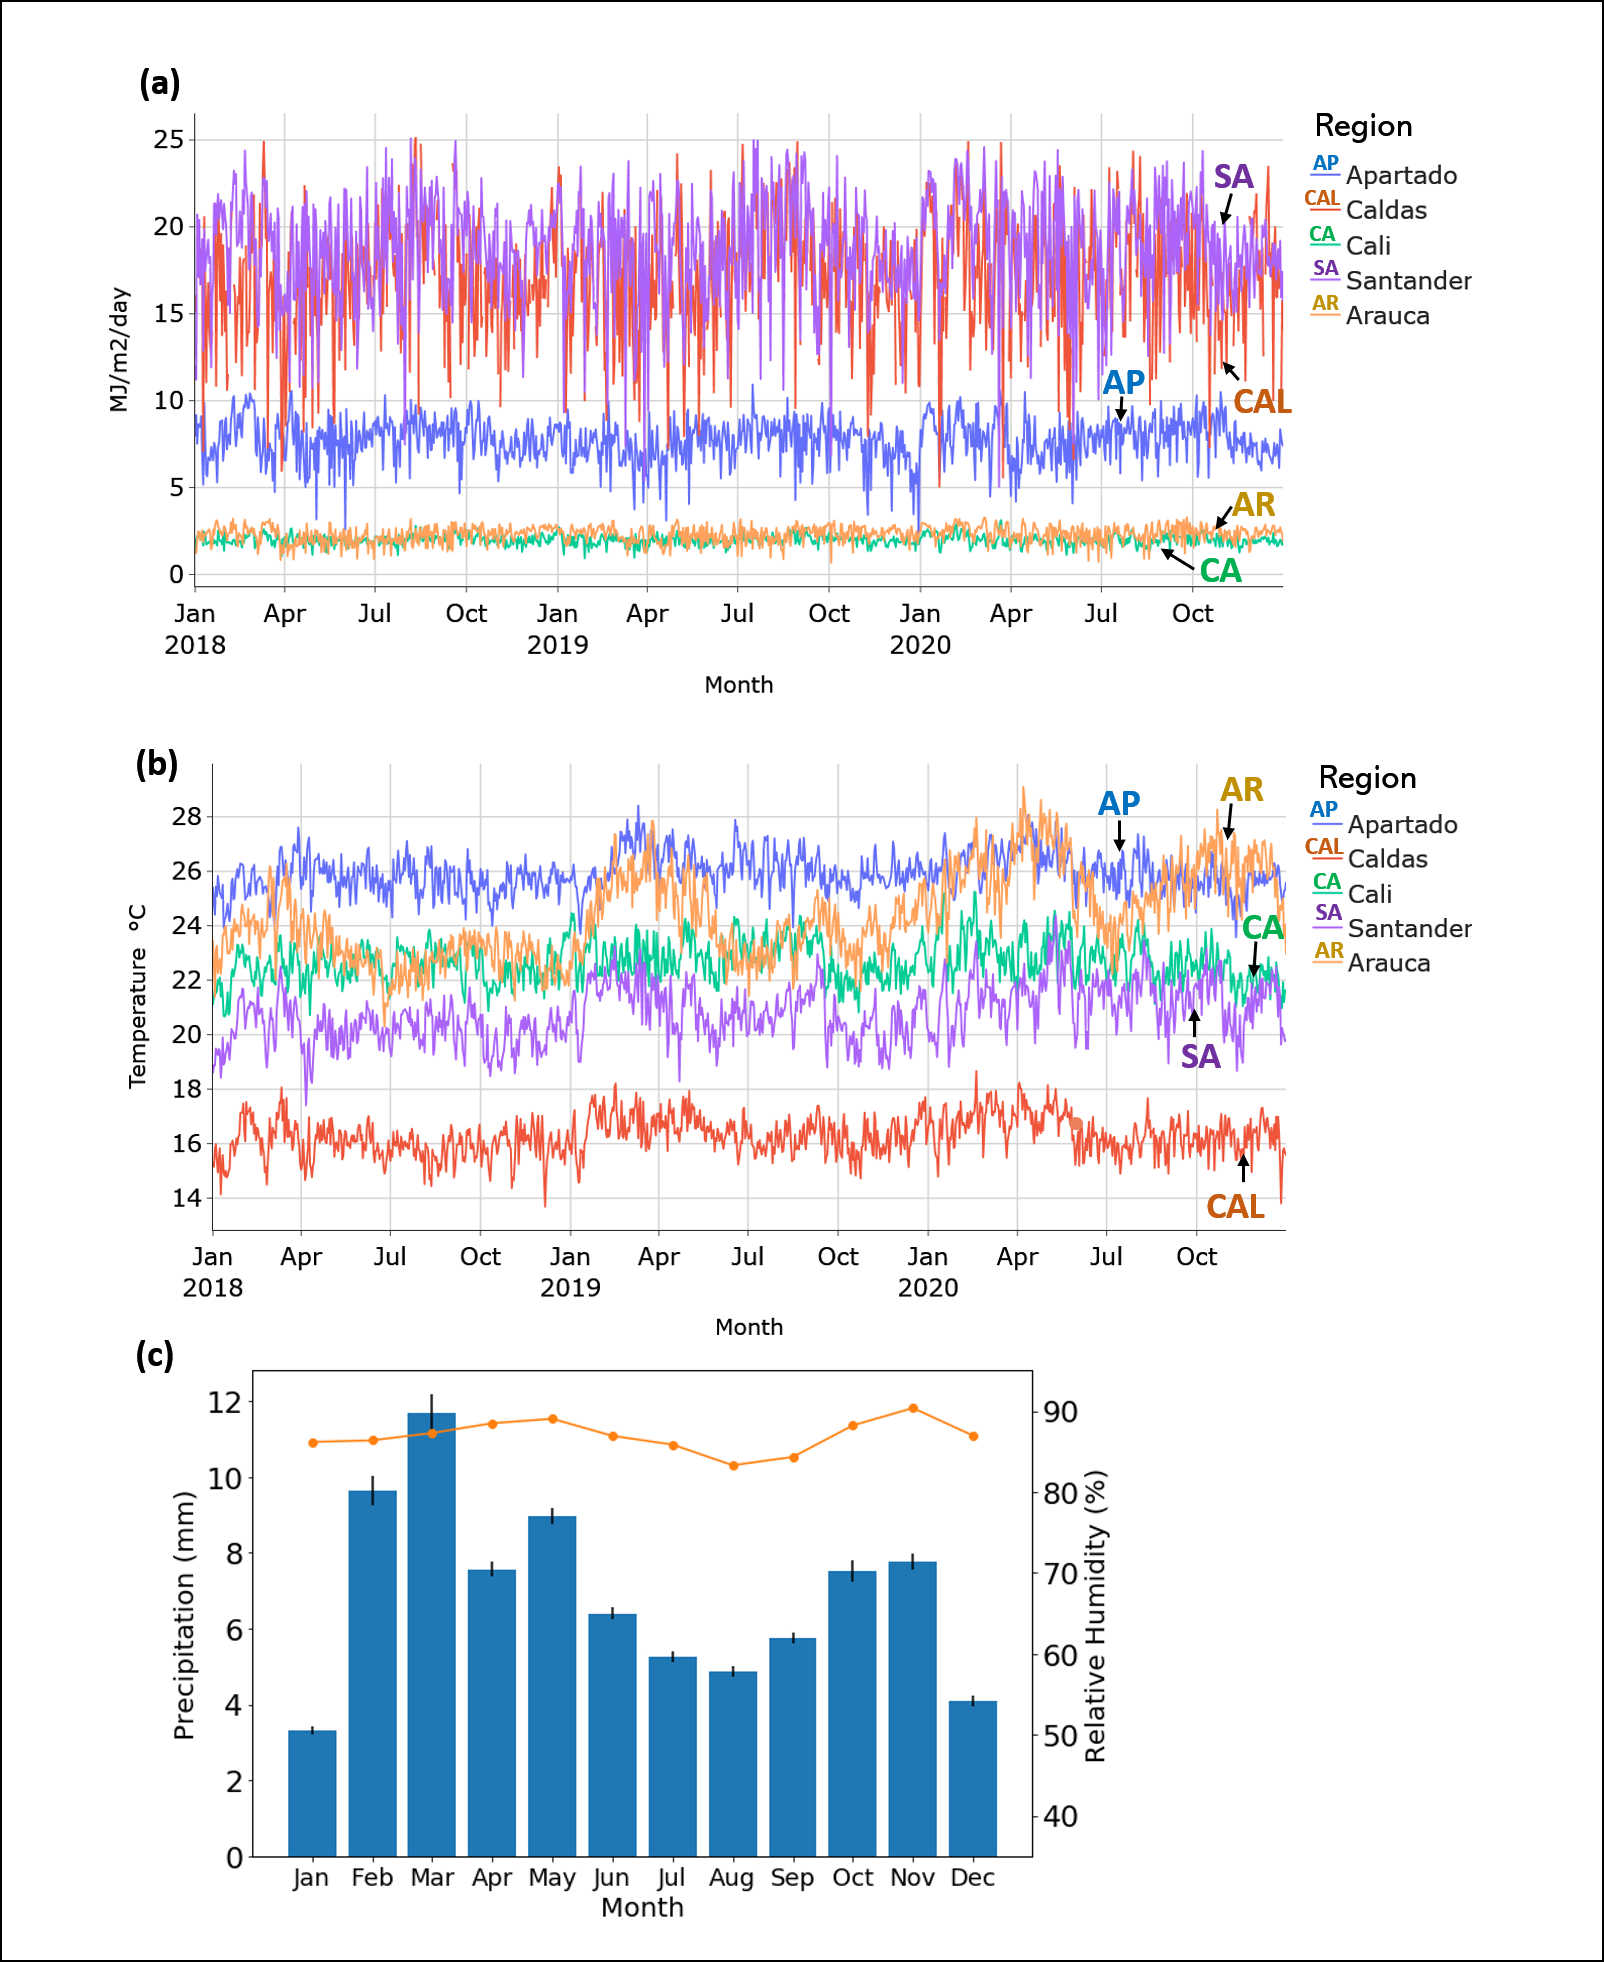
\includegraphics[scale=0.4]{images/clima.png}
	\caption{\footnotesize {Colombian weather conditions. \\}}	
	\label{fig:temp}
	{\footnotesize (a), Available photosynthetic solar radiation (PAR). (b), Daily average temperature  (c), Monthly average of precipitation (bars) and relative humidity (dotted line) from 2018 to 2021 }
\end{figure}
\newpage



\subsection{Inputs and Data Acquisition }

In order to model the phenology of the cacao fruit, linked to collected field data, the cacao model required specific input variables such as Flowering Date (FD), Daily Solar Radiation (SRAD), Daily Maximum and Minimum Temperature (TMAX, TMIN) and Daily Precipitation, specific to a particular agroclimatic region. FD was extracted from the field data, corresponding weather data linked to geographical region was sourced from the POWER Data Access Viewer \citep{nasapower}, from January 01 of 2018 to December 31 of 2020 (Fig.\ref{fig:yield}, b). Weather data was processed using R (R 1.4 version) \citep{Rstudio2020}. 

Since cacao yield depends on the successful development of flowers to form ripe pods, the current view from Colombian farmers (personal communication with Fedecacao)  is that the highest flowering season occurs in September and January which suggests that harvest occurs in March and July. These communication were given through weekly online meetings of KOCOLATL project.  However, the field data collected from Fedecacao suggested that flowering and pod production were not constant for all the locations. For example, pod harvest in the Caldas farm increased in May, and from October to December, and decreased from January to March.  The Arauca and Apartado farms reported highest yield in the months of January, July, November and December. The Santander farm had picks of production in March, May and September (Fig.\ref{fig:yield}, b). 


\begin{figure}[h]
	\centering
	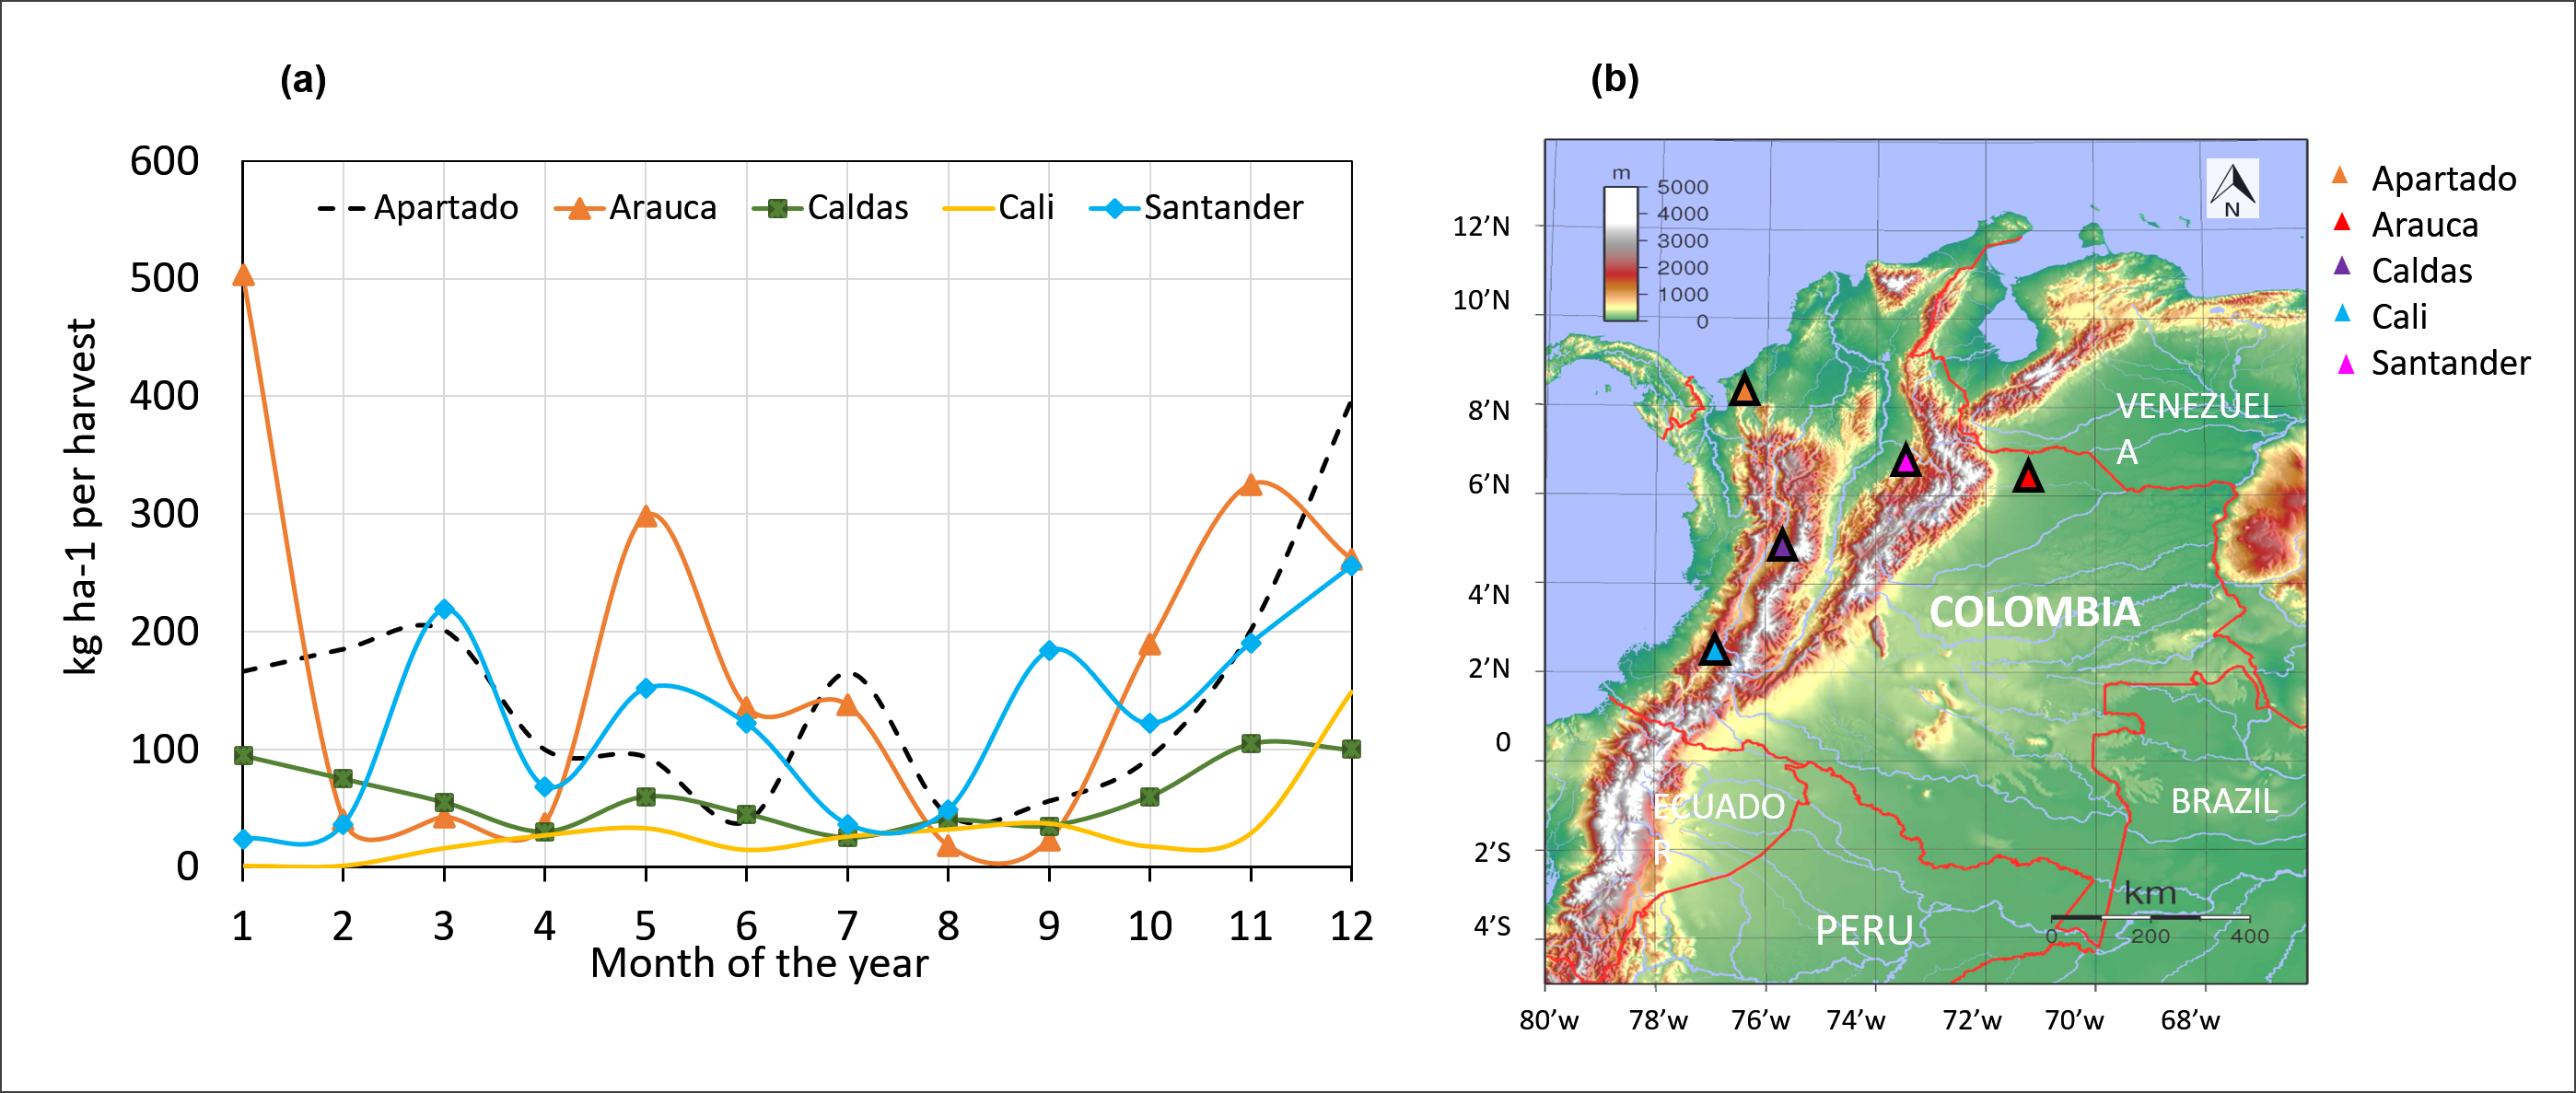
\includegraphics[scale=0.3]{images/map.png}\\
	\caption{\footnotesize {Cocoa production  of five farms in different regions.\\}}
	\label{fig:yield}
	{\footnotesize (a) Map showing the regions where farms are located.  (b) Production per month (2019 - 2020) of five farms.}\\
\end{figure}


\subsection{Thermal Time for Pod Harvest Date Identification}

The cumulative sum of daily temperature from a reference day 0 is defined as \emph{Thermal time} and  its units of measurement are in days degrees (days $^\circ$C). That starter point of 0 days $^\circ$C generally is the planting date \citep{Ritchie1991} but as indicated earlier, our cacao model used FD as the starting point. Thermal time for the development of a cultivated plant may consider the base temperature (T$_{b}$), which is the minimum temperature required by cacao plants to grow. In addition, T$_{b}$ can vary between cultivars \citep{Slafer1995, Daymond2008}. For cacao the vegetative growth T$_{b}$ has been reported between 18.6 and 20.8 $^\circ$C \citep{Daymond2008}. Nevertheless, the pod growth  has a lower T$_{b}$ which range between 9 and 12.9 $^\circ$C \citep{Daymond2008, lahive2019}. We calculated the cacao thermal time with a pod growth T$_{b}$ of 10 $^\circ$C because it is the absolute minimum temperature for cocoa growing in South America reported by \cite{Erneholm1948}, in \citep{lahive2019}.    
 
The thermal time required for the cacao crop model was characterised for each location starting from FD (0 days $^\circ$C) to harvest date (180 after flowering = 6 months), as farmers used to harvest by calendar days. Thus, the cacao model predicts the maturation day to harvest pods. It can vary depending on temperature variations.  Thermal time was calculated using the equation \ref{equ:tem}. Where tt is the cumulative sum of the daily temperature (T$_{i}$) and T$_{b}$ for cocoa is 10$^\circ$C.

\begin{equation}
Thermal~time~(tt) = \left\lbrace\begin{array}{c} \sum_{i=1}^{n} T_{i} - T_{b} \\
\vspace{0.2cm}\\ 
0,\hspace{0.2cm} Flowering~date\end{array}\right.
\label{equ:tem}
\end{equation}


\subsection{Model Calibration}

Calibration of any crop model is conducted typically for a particular cultivar and agroclimatic region \citep{Crout20142}. The cacao model was calibrated, for five particular regions and two cultivars, by sequentially modifying the physiological variables and then comparing the degree of similarity between observed and predicted data \citep{Crout2008chapter, Zao2019simple,Camargo2019aquacropr, Bai2020}. The original code of SIMPLE model from \citep{Zao2019simple} was modified into the cocoa model. The process of calibration stops when the distance between observed and simulated data doesn't improved any longer. The cacao model has seven input files where new cocoa crop data are provided. Files in the list below can be edited to define the features of the new cultivars or experiments. Since cacao phenology has not been simulated with the SIMPLE model, cacao physiological information such as Leaf Area Index (LAI) for shade plants \citep{Agele2016, Soltani2012, zuidema2005,Baracaldo2014} and Harvest Index (HI) \citep{Quintana2015} were extracted from the current literature and verified with Fedecacao cacao experts. Other variables such as Radiation Use Efficiency (RUE) \citep{Fletcher2013RUE,Bonhomme2000} were based on the perennial crops banana and cotton which have been calibrated previously in the SIMPLE model \citep{Zao2019simple} using RUEs of 0.8 and 0.85 for banana and cotton, respectively. As cocoa trees usually grow under shadow \citep{lahive2019}, we estimated by trial and error that lower RUE values (between 0.7 and 0.5 g MJ$^{\mathbf{-1}}$ m$^{2}$) than those utilized by \cite{Zao2019simple}, was a most ideal range  (table \ref{tab:reparam}). 

\subsection{Parameters}

This cocoa model has three parameters which vary by region (table \ref{tab:reparam}): The thermal time required for harvest after the FD (Tsum) , the Radiation Use Efficiency (RUE) and yield observed on field. Physiological parameters in table \ref{tab:Treaparam} are  common  for all the regions studied. These parameters were calibrate for cultivars ICS95 and CCN51 considering a range of time of 200 DAF to harvest day, even thought farmers collect the pod at 180 DAF. Heat and water stress parameters were not considered as this study was not assessing biotic o abiotic stresses.

\begin{table}[h!]	
	\caption {\footnotesize {Cocoa crop parameter values used per region.}}
	\label{tab:reparam} 
	\centering
	\begin{small}
		\begin{tabular}{l c c c }
			\hline
			{\bf Region }&{\bf Tsum }&{\bf RUE}&{\bf Yield$^{*}$}\\
			\hline
			Apartado   & 2906 & 0.6 & 3378  \\
			Arauca   & 2764 & 0.7 & 3981  \\
			Santander & 2016 &0.6 & 2687 \\
			Cali   & 1912 & 0.5 & 1900  \\
			Caldas   & 1192 & 0.6 & 740  \\
			\hline
		\end{tabular} \\
		{\footnotesize RUE Radiation use efficiency (above ground only and without respiration)g MJ$^{\mathbf{-1}}$ m$^{\mathbf{2}}$\\$^{*}$ Yield observed kg ha$^{\mathsf{-1}}$ per year. } 
	\end{small}
\end{table}


\begin{table}[h!]	
	\caption {\footnotesize {Parameter values used to run the cacao model.}}
	\centering
	\label{tab:Treaparam} 
	\begin{small}
		\begin{tabular}{{l l l}}
			\hline
			{\bf File }&{\bf Variable name }&{\bf Value}\\
			\hline
			&SoilName & Loamy sand4\\
			&InitialFsolar & 0.01\\
			Treatment&Weather & KOKO (.WTH file name)\\
			&CO$_{2}$ & 400 ppm\\
			&SowingDate &Flowering Date (FD)\\
			\hline
			&Crop cycle DAP & 200 days\\
			&LAI & 1.8 \\
			Observation&FSolar& 0.70\\
			&Biomass & 40kg dry mass per plant\\
			\hline
			&Harvest index & 0.3\\
			Cultivar&150A & 680 $^\circ$C day \\
			&150B & 680 $^\circ$C day \\
			\hline
			&Tbase & 10$^\circ$C\\
			&Topti & 26$^\circ$C \\
			Species&MaxT & 35$^\circ$C \\
			&ExtremeT & 40$^\circ$C  \\
			&CO$_{2}$RUE & 0.09$^\circ$C  \\			
			&S-water & 0 ARID index \\
			\hline			
		\end{tabular} \\ 
	\end{small}
	{\footnotesize S-water is associated drought stress evaluations ranging from 0 (no water shortage) to 1 (extreme water shortage) \cite{Zao2019simple} }
\end{table}
\newpage


\subsection{Evaluation of Model Performance}

The cocoa model performance was evaluated by comparing simulated values cocoa yield with those reported by Fedecacao from cocoa plantations, using the statistical index of Relative Root Mean Square Error (RRMSE)  in the equation \ref{equ:RRMSE}, where n is the total number of observations, Y$_{i}$ corresponds to observed value from field and X$_{i}$ is the predict value from the model.\\

\begin{equation}
RRMSE= \sqrt{\frac{\frac{1}{n}  \sum_{i=1}^{n} (Y_{i}-X_{i})^{2}}{\sum_{i=1}^{n} X_{i}^{2} } } \times 100\% 
\label{equ:RRMSE}
\end{equation}



\section{Results}

\subsection{Weather Conditions Over Flowering Time }
Figure \ref{fig:heat} shows the Pearson correlation to study the weather data of the flowering time over the months of flowering  (monthF), month of harvest (monthH) and their final yield (fruit\_kg). The results showed that thermal time T$_{b}$ (ttb) is correlated (P = 0.52) with daily average temperature and maximum temperature (TMAX) and  temperature minimum (TMIN) and Dew Frost Point at 2 meters (T2MDEW) with  a correlation coefficient of 0.60. The wind (WS2M) is correlated with ttb with 0.57. However, less clear correlations were found of monthF  with T2MDEW, relative humidity (RH), WS2M and rain. Although, farmers stated that the number of flowers pollinated decrease by months where wind and rain are high (personal communication with Fedecacao), our analysis  (Fig. \ref{fig:heat}) could not show a correlation between flower shedding and high wind or rain because information on number of  flowers at FD was not part of the field data collected. 


\begin{figure}[h!]
	\centering
	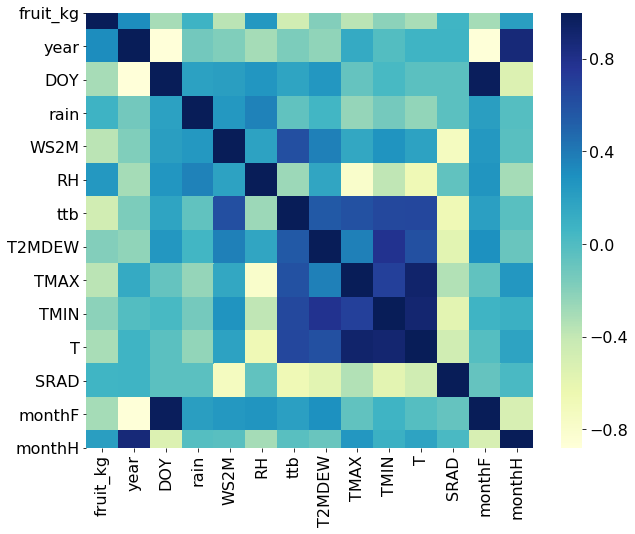
\includegraphics[scale=0.2]{images/heatm.png}\\
	\caption{\footnotesize {Pearson correlation average weather variables and FD for five locations in Colombia. \\}}
	\label{fig:heat} 
	{\footnotesize Numbers in the squares are the correlation coefficients }
\end{figure}
\newpage

\subsection{Thermal Time }

Thermal time characterisation was made considering 180 DAF for each location. The box-plot in the figure \ref{fig:ttbox} shows the data distribution where boxes indicate the range of the central 50\% of the total data per region, the central line in the box is marking the median value and lines draw out from each box mean the range of the remaining data. Therefore, this boxplot shows differences between locations as was expected following the tendencies of the temperature of the figure \ref{fig:temp}, (b), where Aparatado, Arauca and Cali had greater temperatures than Santander and Caldas. 

Therefore, Apartado and Arauca had the highest temperatures and consequently the highest thermal time values with 2909 and 2764 days$^\circ$C  respectively. Caldas had the lowest values with 1173 days$^\circ$C. Meanwhile, Cali and Santander presented similar thermal time around 2000 $^\circ$C (table \ref{tab:reparam}). The accumulated temperature during the pod development (fig.\ref{fig:ttbox}) depends on the region where cocoa is cultivated, and the variety planted. Thermal time values are also proportional to the yield reported on field (table \ref{tab:reparam}). \\

\begin{figure}[h!]
	\centering
	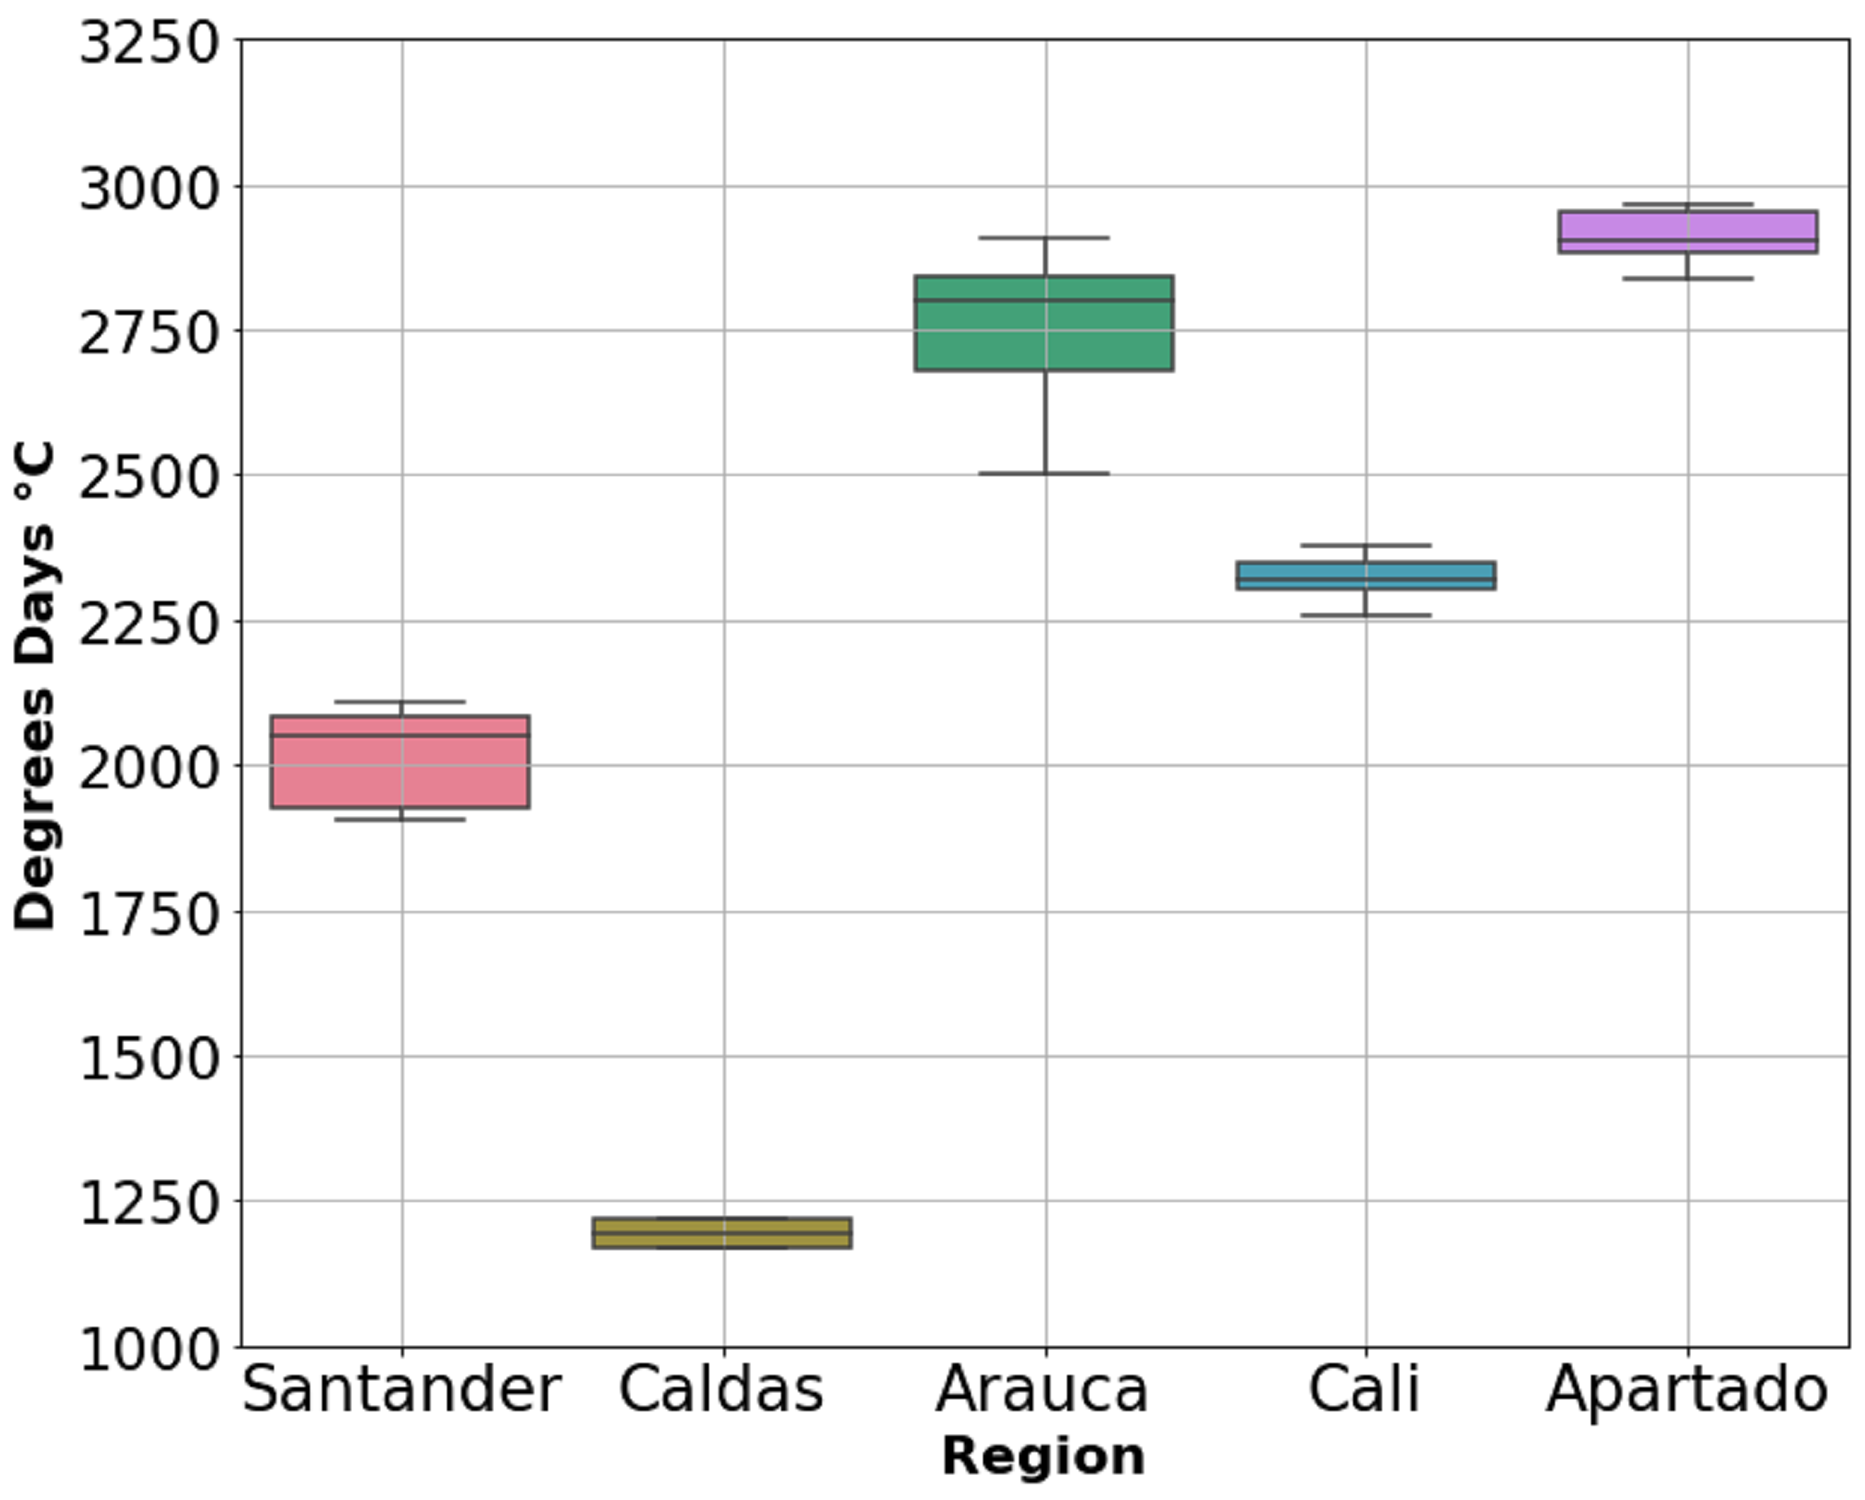
\includegraphics[scale=0.2]{images/ttbbox.png}\\
	\caption{\footnotesize {Cocoa yield and thermal time characterisation at 180 DAF.\\}}
	\label{fig:ttbox}
\end{figure}



\subsection{Model Validation}

Biomass production of the aerial part of the cacao tree was simulated which include every organ of the plant that is over the soil surface. It is important to calculate how much biomass from the crop aerial is partitioned to the cacao pods according to the harvest index (HI) (table \ref{tab:Treaparam}) as this quantity will correspond to the weight of cacao seeds.  

Figure \ref{fig:m1} (a) shows the daily biomass growth rate for five agroclimatic regions. Biomass simulation is affected by the solar radiation, RUE \citep{Fletcher2013RUE,Bonhomme2000}, daily temperature, atmospheric CO$_{2}$ concentration (ppm) and the fraction of solar radiation intercepted by a tree of cocoa during the fruit development (fSolar) (fig. \ref{fig:m1}, b). We did not compare predicted and observed Biomass as there were not field data corresponding to absorption of solar radiation by the plants or of biomass production. Figure \ref{fig:m1} (c) also shows that the daily biomass growth rate increased proportionally with the yield production, suggesting that it was possible to calculate the final yield as the product of accumulated biomass at the harvest day and HI = 0.3 (Equ.\ref{equ:HI}).

\begin{equation}
Cocoa~yield = Accumulated~ biomass~\times~ HI \\
\label{equ:HI}
\end{equation}


The fraction of solar radiation intercepted by cacao trees (fSolar) was also simulated for the fruit development cycle. The relation of fsolar and is strongly related with RUE \citep{Fletcher2013RUE,Bonhomme2000}, LAI and hence the senescence of the canopy leaves \citep{lahive2019, Danner2015, Soltani2012, Romero2017, Vina2011, Zao2019simple}. Results in the figure \ref{fig:m1} (b) showed that all regions had a maximum fSolar of 0.94, except from Caldas whose peak fSolar was at 0.76.  fSolar-max was faster reached in the regions of Apartado and Arauca. These fSolar-max values of solar radiation intercepted for photosynthesis, lasted differently depending on the region and their solar radiation (Fig.\ref{fig:temp}, a) : Apartado 66 days  from  69 to 135 DAF,  Arauca 61 days from 72 to 133 DAF, Cali 38 days from 83 to 121 DAF,  Santander 24 days from 92 to 116 DAF and Caldas 2 days at 125 DAF. fSolar declined and hence the interception of solar radiation until the pod harvest day. 

The RRSME has been used before to evaluated other crop model simulations \citep{Zao2019simple, Bai2020}. Our results of cocoa yield simulation (kg ha$^{-1}$ per year) and validation (table \ref{tab:reparam}) achieved a final RRMSE of 7.2\%  fit between simulated and observed data (fig. \ref{fig:m1}, c). \textcolor{blue}{ The low RRMSE  indicates the simplicity of the Cacao model to simulated cacao  yield. Although, the original SIMPLE model can be used to asses heat and water stress, our cacao model calibration  did  not accounted biotic (pest and diseases) and abiotic (heat or water stress) factors that could have significant effects on the cacao production.}

Individual errors per region are presented in table \ref{tab:error}, where the best fit of the calibration model for yield prediction  was for crops in  Apartado and the highest error was calculated for Caldas crops.  
 The model responded to the variations of temperature and solar radiation. Therefore, the highest  yield values simulated were obtained for Arauca over 4000 kg ha$^{-1}$, followed by Apartado Santander with yields over 2000 kg ha$^{-1}$.  The lowest yield was simulated for the Caldas region with less of 1000 kg ha$^{-1}$ . Final yield in the model was calculated as the product of biomass of aerial part and harvest index (HI) \citep{Zao2019simple, Amir1991}, where the HI is similar to the CropSyst \citep{STOCKLE2003} and AquaCrop \cite{Steduto2009}. 

\begin{figure}[h!]
	\centering
	\includegraphics[scale=0.4]{images/outmodel.png}
	\caption{\footnotesize {Model predictions. (a) Biomass aerial part. (b) Interception of solar radiation. (c) Yield. Crop cycle close to 180 DAF (vertical red line) base on figure  \ref{fig:ttbox}.  \\ }} 
	\label{fig:m1}
\end{figure}
 

\begin{table}[h!]	
	\caption {\footnotesize {Summary of relative root mean square error RMSE for yield prediction using The cocoa model.}}
	\label{tab:error} 
	\centering
	\begin{small}
		\begin{tabular}{l c c c c c c}
			\hline
			{\bf Region }&{\bf Apartado }&{\bf Arauca}&{\bf Santander}&{\bf Cali}&{\bf Caldas}&{\bf Overal}\\
			\hline
			RMMSE \%  & 3 & 6.05 & 10.06&8.5&14.90&7.2 \\
			\hline
		\end{tabular} \\
	\end{small}
\end{table}
\newpage

\subsection{Predicting Optimal Pod Harvest Day }

Farmers practice of empirically harvesting is about counting  180 DAF (6 months) by calendar without taking into account weather changes or physiological features of cacao cultivars.
Since our cacao model was fitted to predict optimal pods harvest date, we compared model predicted dates against the usual 180 days that growers and experts count after the FD. Figure \ref{fig:dayH} shows observed day of harvest (180 DAF) independently of the region. All the regions except Santander, presented the earliest predicted harvest when the FD was between December and February. The fruit can be ready to harvest before or after 180 DAF depending on the environmental condition per region. The results in the figure \ref{fig:dayH} demonstrated that the traditional way to harvest which is always at 180 DAF, it is not having account physiological and environmental conditions that can be affecting the pod maturation. Thus, when the fruit development was simulated the maturity day in Cali and Caldas were from 3 to 12 and 4 to 23 days before 180 DAF. Apartado presented the most similar predicted dates of harvest to 180 DAF with 170 to 182 DAF. The pod may be harvest in Arauca from 165 to 193 DAF, Santander from 165 to 183 DAF, ten days less than in Arauca for the same months of flowering of July and August of 2019 . Only Arauca presented longer crop cycles when the FD was between during that period of time. This means that Arauca had bigger variation of temperature between months. To summarize, depending on which month of the year cacao trees are flowering,  the number of days to reach the harvest of ripe pods vary more or less 180 days. For example, if cacao trees in Caldas are flowering in January, pods will be ripe to harvest in about 158 days proximately  (table \ref{tab:harvest}). 
 
\begin{figure}[h!]
	\centering
	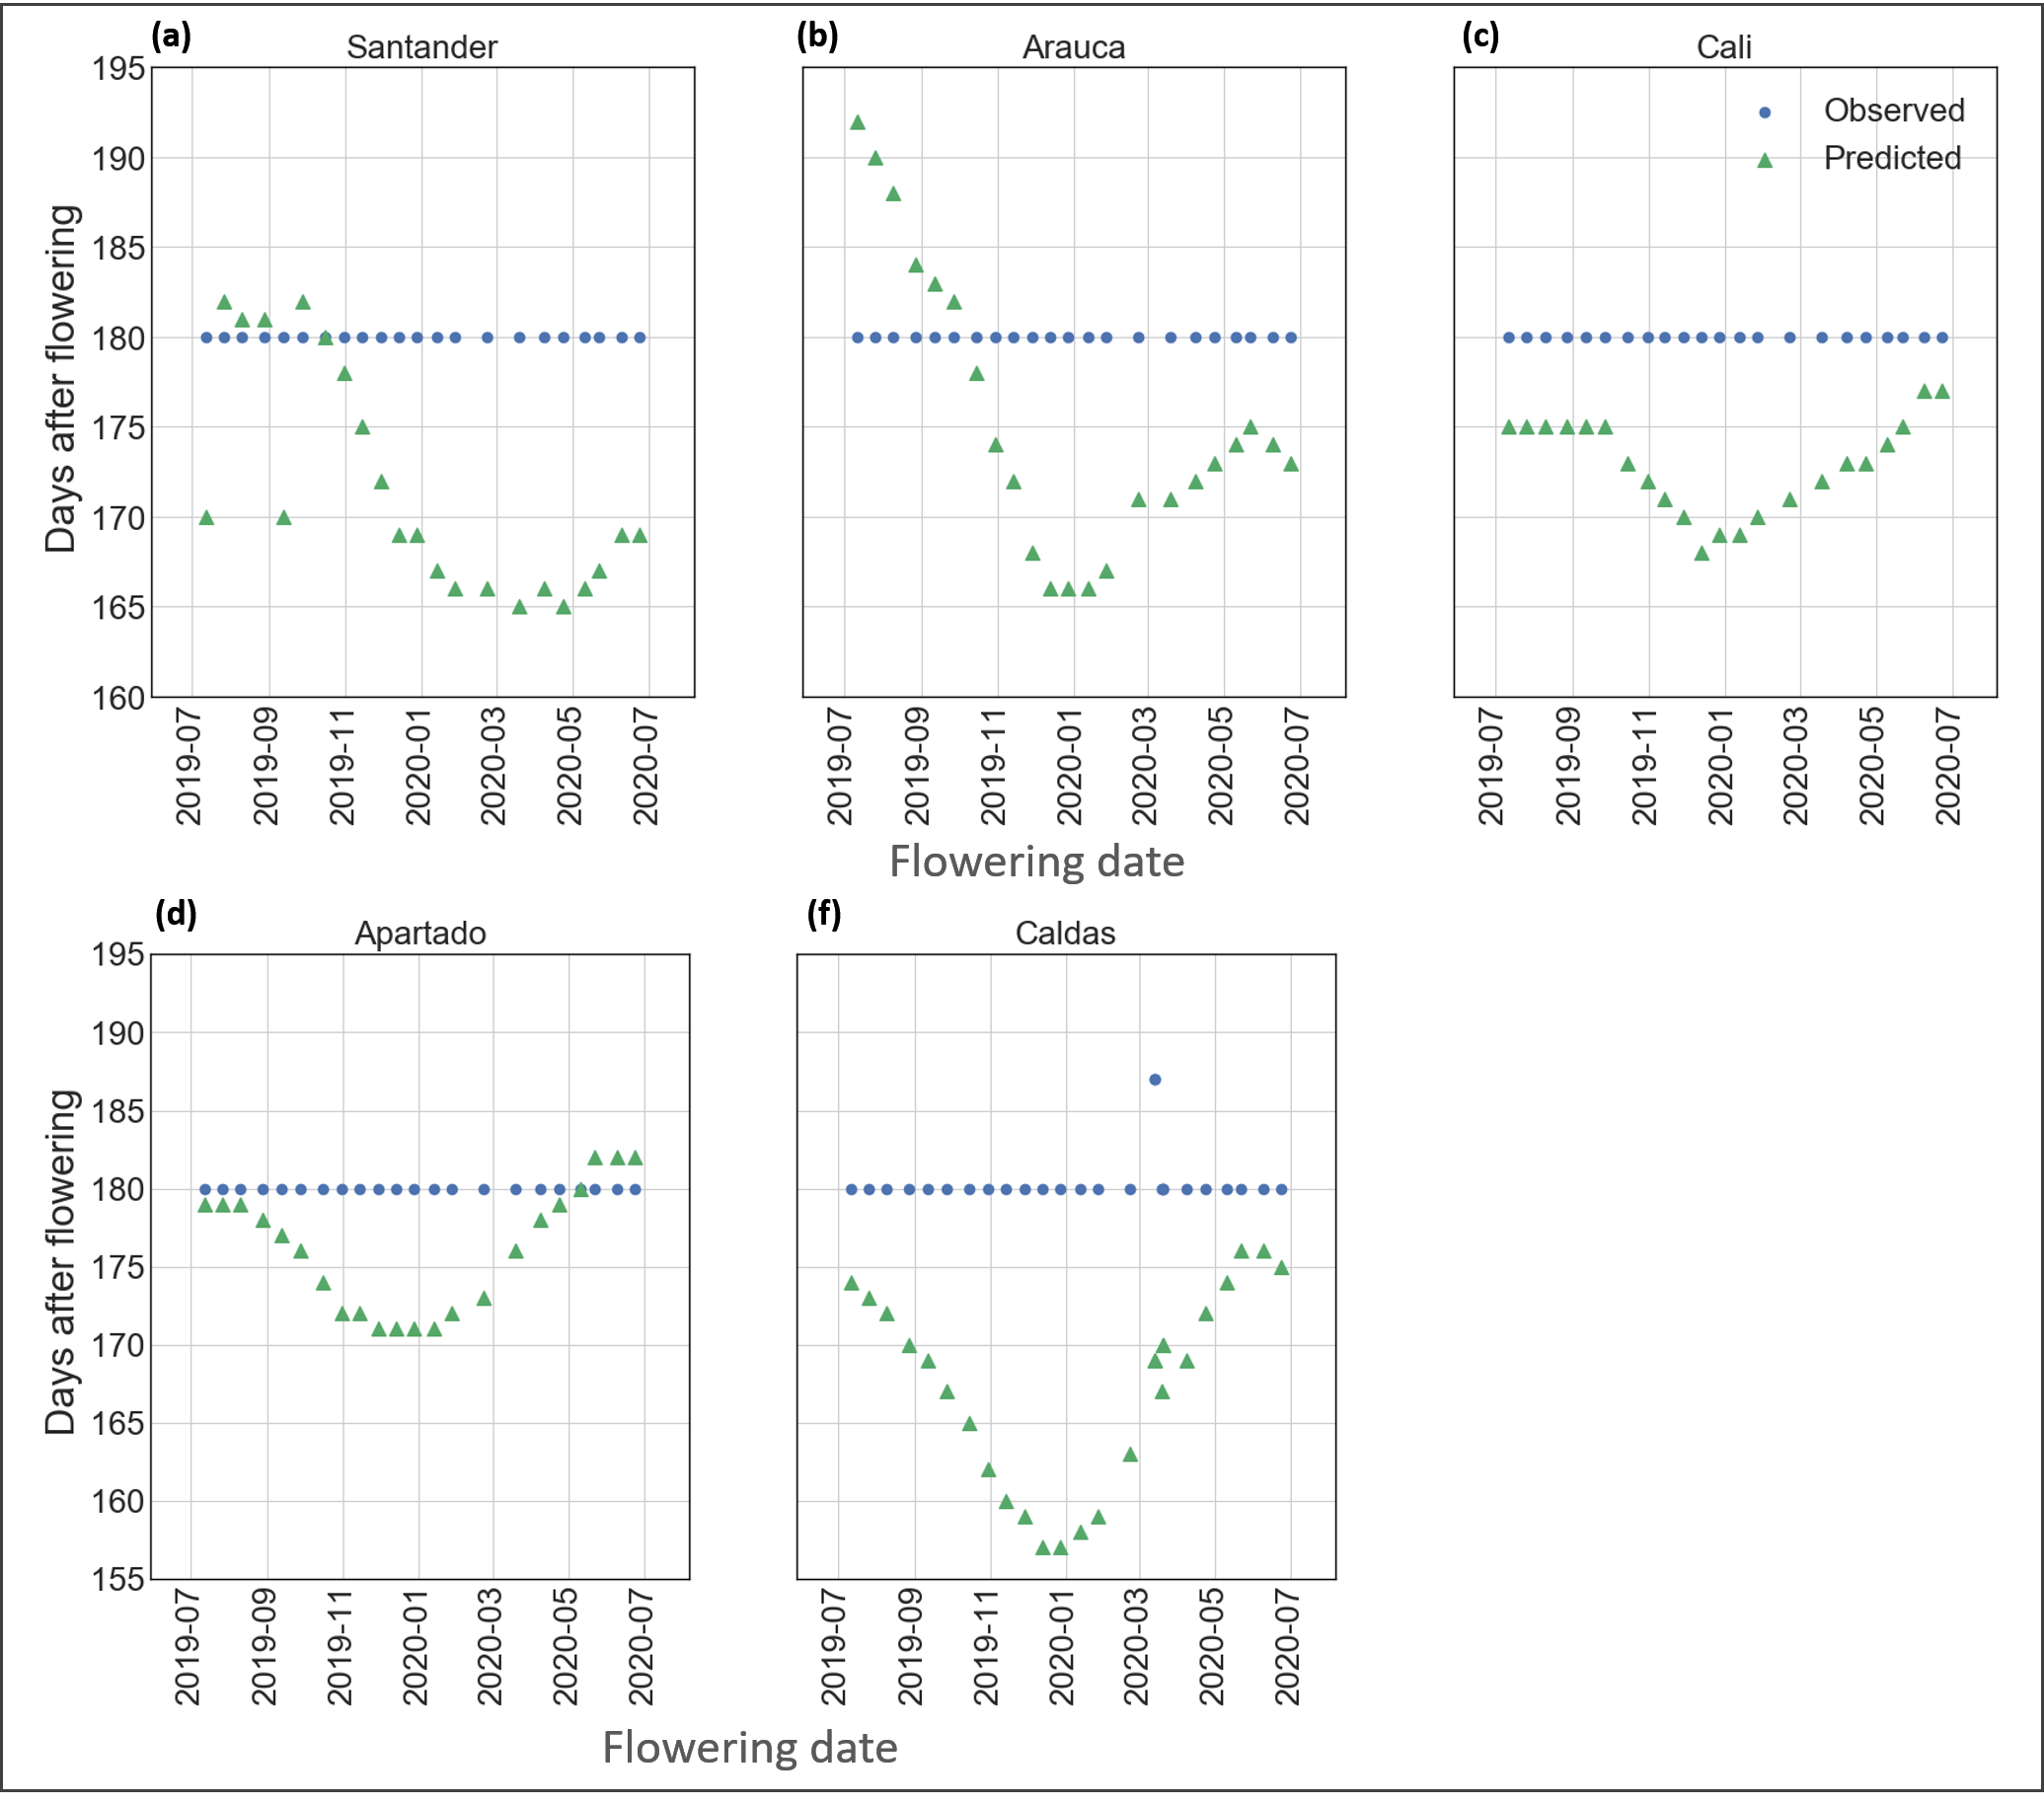
\includegraphics[scale=0.4]{images/RegionHarvest2.png}
	\caption{\footnotesize {Cacao harvest day prediction from FD for Apartado , Arauca, Caldas, Cali  and  Santander. DAF = Days After Flowering. FD = Flowering Date. \\ }} 
	\label{fig:dayH}
\end{figure}.
\newpage

\begin{table}[h!]	
	\caption {\footnotesize {Average of days to harvest according to the month of flowering.}}
	\label{tab:harvest} 
	\centering
	\begin{small}
		{\def\arraystretch{2}\tabcolsep=10pt
		\begin{tabular}{l c c c c c }
			\hline
			{\bf Month }&{\bf Santander }&{\bf Arauca}&{\bf Cali}&{\bf Apartado}&{\bf Caldas}\\
			\hline
			January    & 166.5 & 166.5 & 169.5& 171.5 & 158.5 \\
			February   & 166 & 171 & 171 & 173 & 163  \\
			March      & 165 & 171 & 172 & 176 & 167  \\
			April      & 165.5 & 172.5 & 173& 178.5 & 170   \\
			May       & 166.5 & 174.5 & 174.5&  181& 175   \\
			June      & 169 & 173.5 & 177&  182& 175.5   \\
			July      & 176 & 191 & 175& 179 & 173.5  \\
			August    & 181 & 186 & 175& 178.5 & 171   \\
			September   & 176 & 182.5 & 175& 176.5 & 168   \\
			October    & 179 & 176 & 172.5& 173 & 163.5   \\
			November   & 173.5 & 170 & 170.5&171.5 & 159.5   \\
			December   & 169 & 166 & 168.5& 171 & 157  \\
			\hline
		\end{tabular} \\
	}
		{\footnotesize Days to harvest cocoa after flowering are approximate, as these are results from the cocoa model simulations. Calibration was based on FEDECACAO reports from 2018 to 2020. } 
	\end{small}
\end{table}
%%%%%%%%%%%%%%%%%%%%%%%%%%%%%%%%%%%%%%%%%%

\section{Discussion}


Cacao is one of the most economically important crops in Colombia. In 2016 Colombia produced a historical of 56K tons, up from 35K ten years ago, and over the same period, imports decreased from 12.8K to 488 tons (FAOStat). Cacao has been fundamental in the transformation of the rural economy dependent on illicit crops. As such, Cacao is called the "peace crop", nominated by  Colombia's President and 2016 Nobel peace prize winner, Juan Manuel Santos, and by the President of the Association of Cacao Growers (Fedecacao). Although Colombian cacao has the potential to be in the high value markets for fine flavour, the lack of expert support as well as the use of traditional, and often times suboptimal, technologies makes cocoa production negligibly. 

\textcolor{blue}{This study reports the cacao model which was calibrated for five agroclimatic regions in Colombia. The model simulates crop development, growth and yield, and predicts the maturation day when the fruit is likely to be ready for harvest.  The purpose of this model was to help farmers achieve  higher quality cacao beans by providing them with a tool that not only predicts optimal harvest date but also estimated a potential yield and biomass . The low RRMSE for yield prediction indicates the simplicity of the Cacao model to simulated cacao  yield. Although, the original SIMPLE model can be used to asses heat and water stress, our cacao model calibration  did  not accounted biotic (pest and diseases) and abiotic (heat or water stress) factors that could have significant effects on the cacao production.  Santander and Caldas have the  highest solar radiation but the lowest temperature. In contrast , Arauca and Apartado have the  highest temperature but the lowest solar radiation
Weather analysis could not show a correlation between flower shedding and high wind or rain because information on flowers was not part of the field data collected. 	The growth cycle was simulated in terms of thermal time which was defined for the five regions tested, given the dependency to the crop model to predict the harvest day according to the weather variations while fruit are growing.  The thermal time calculation was defined base on  180 DAF because farmers cut the pods by calendar days. Our results showed how the harvest day can vary depending on the accumulate temperature during each specific crop cycle simulated (Fig. \ref{fig:dayH}).
}



\subsection{Weather Effects over Flower Stability and Pollination}

Our analysis of weather variables (Fig. \ref{fig:heat}) could not show a correlation between flower shedding and high wind or rain because information on flowers was not part of the field data collected. However, farmers stated that the number of flowers pollinated decrease by months where wind and rain are high. High winds can affect the availability of tiny flies pollinators from Diptera order and from the families of of the biting midges \textit{Ceratopogonidae},  genus  \textit{Forcipomyia} \citep{Saunders1959, kaufmann1975, sotomayor2020} to reach the cacao flowers. However, the stability of cacao flowers is influenced by seasonal wheather conditions (abiotic) and pollination (biotic) \citep{Frimpong2014}. Therefore, pollinator population should be coincidence with the phenology of the flowering cacao trees \citep{Young1983, Young2012}. Flower opening is very well synchronised between the cohorts of mature flowers opening each night \citep{Niemenak2010}. The flowers open at almost exactly the same time and rate, irrespective of their position on the trunk. Thus, unfertilised flowers abscise from the trunk approximately 1 day after flower opening  \citep{Niemenak2010}. Hence more than 90\% of unpollinated flowers fall or abscised within 32 hours after  anthesis \citep{Aneja1999}. Abscission processed of  flowers are mainly controlled  by  three  hormones: auxin, ethylene, and abscisic acid (ABA) \citep{Aneja1999}. Ethylene generally promotes abscission because it may  inhibit the transport of auxin from the leaf blade, which allow the action of ABA to promote the fall of flowers \citep{Beyer1975}. In general, environmental conditions can also  stimulate   to  a  decrease  the  auxin/ethylene relationship \citep{Aneja1999}.

When analysing the data from  Santanter region, we showed that the number of successful flowers pollinated to produce final yield could be affected by rain, TMAX and wind. Nevertheless, a better field data tracing flowers development is essential to understand if it is a mechanical or physiological effect.  \cite{Frimpong2009, Frimpong2011} indicated that the numbers of cocoa pollinators were reduced during the dry season, but increased in the wet season. This, could be due to midges need a moist environment to develop \citep{Frimpong2014}, which is difficult during the dry season as cocoa leaves create a dried ground mat \citep{Frimpong2009, Frimpong2014}. Moreover, the lack of water during dry seasons may reduce the nutrients uptake provoking the massive flower drops \citep{Vaughton2017}.  For future studies, wind could be included in the cocoa model as an input to simulate this mechanical effects over number of flowers. In general, field data regarding counting flowers pollinated by month should be better reported for the region here studied. 

\subsection{Thermal Time for Harvest Day Predictions}
We define the thermal time required to harvest cocoa pods for five Colombian regions as maturation of the fruit is related with temperature during the growth cycle \citep{lopez2018}. Previous studies have calculated thermal time for  different cocoa cultivar in Brazil and Ghana \cite{Daymond2008}. They also confirm that the fruit maturation time decrease in with an increase in temperature as was presented on others researches \citep{Alvim1974, End1991, Daymond2008}. the effects of temperature and solar radiation on fruit growth and development was previously studied by \cite{Daymond2008}, showing that crop under higher temperatures thought the crop cycle induce greater fruit losses because of physiological maturation (cherelle wilt). When the fruit is mature, seeds are able to germinate  \citep{lopez2018}. \textcolor{blue}{However, when ripe fruits stay for a longer time on the tree without be harvested  on the right moment, seeds can germinate inside the pod damaging  cacao production for high-quality taste and affecting the final yield. }

Our results showed that the hotter regions such as Apartado and Arauca presented higher thermal time values (Fig. \ref{fig:ttbox} and \ref{fig:temp}). Even though, Arauca had very low values of SAR but very high temperatures, this may be caused by clouds cover. The opposite can be seen for Caldas and Santander. These, extreme relations T/SAR can compensate the crop efficiency, for example in Santander (Fig. \ref{fig:m1}).  The thermal time calculation was defined base on  180 DAF because farmers cut the pods by calendar days. Previous studies stated that evaluating the level of knowledge of growers regarding cocoa crop management, showed that the harvest was in the group of activities that presented the lowest level of information by the farmers \citep{Gutierrez2020}. That is why, these results present important temperature boundaries to predict fruit maturation day. Therefore, may be other environmental factors that should be studied for further research. 

\subsection{Cocoa Crop Model Simulations}
Although cocoa is a relevant crop and there is an extensive agronomic literature, there is only one physiological crop model specific for cocoa so far. The (SUCROS-Cocoa) developed by \cite{zuidema2005}. However, the code was not easy available for adaptations. In contrast, the SIMPLE model has an open code in R, which we could adapt such a model would be very useful to compare yields and predict harvest date in different climates. As the harvest day was predicted from the FD (Fig. \ref{fig:dayH}, consequently, biomass production and fSolar presented a crop cycle shorter than 180 DAF (Fig. \ref{fig:m1}, a and b). These simulations are coincident with results presented by \cite{lopez2018}, where physiological maturity of coca pod varies from 140 to 162 DAF.  Our results showed how the harvest day can vary depending on the accumulate temperature during each specific crop cycle simulated (Fig. \ref{fig:dayH}). \textcolor{blue} {Harvesting cocoa fruits at the right moment the quality of the seed inside the pod can improve avoiding the germination before collect the pot from  cacao trees.}\textcolor{olive} {An research made by Gallego (2021), cacao clones CCN51 and ICS95 were handed-pollinated and pods were collected at 6, 7, and 8 months of ripeness after pollination. Cacao fruits were harvested from the municipality of Belalcazar, Caldas, Colombia to analyse metabolites related with cocoa quality were more expressed when fruits are collected at 6, 7, and 8 months after flowering.  Results showed that the metabolites that mostly explain the differences between the classes ( metabolites with the highest VIP) are highly overexpressed at month 6 and then decline or under-expressed at the next months.  No significant differences were found in their metabolic profile Between month 7 and 8.
Quality of cocoa is defined by  some metabolites that are associated with flavonoids or colouration. When the expression of flavonoids decrease , indicates  that  metabolites  associated with flavonoids  are being oxidized and metabolites are converted by cells into other less oxidizing metabolites. The colouration does not show a greater difference after month 6. If there is no good  accumulation of flavonoids which are also related with metabolites associated with colouration, the quality of cocoa seed decrease. Ripening is associated with changes in colouration and these in turn with flavonoids so month 6 was ideal for harvesting assuring the high quality of cocoa. } \textcolor{blue} { Therefore, the cacao model can predict with more detail the optimum day to harvest the pod ensuring the quality of the cacao bean  destined for Fine-cocoa products. } 

 
Biomass simulations use cocoa model presented similar predicted values (10000 Kg ha$^{-1}$) for coca drops in Costa Rica using SUCROScocoa \citep{zuidema2005}. Biomass simulations are a common evaluation in crop modells such as Sirius \citep{Crout20142}, SUBSTOR-potato \citep{Raymundo2017} and  DSSAT, CropSyst, STICS and WOFOST \citep{Confalonieri2016}. The approach of this research was focus  on the harvest date prediction, hence the leaves crop cycle was evaluated indirectly this study. The fraction of intercepted photosynthesis active radiation (fSolar) decreased (Fig. \ref{fig:m1}, b) when the senescence of the canopy \citep{zuidema2005}. The relation of fsolar and LAI \citep{lahive2019, Danner2015, Soltani2012, Romero2017, Vina2011, Baracaldo2014} and RUE \citep{Fletcher2013RUE,Bonhomme2000} have widely been reviewed in literature . The  production of photo-assimilates, dry matter and yield can be affected by LAI and RUE reduction \citep{Deblonde2001, Fletcher2013RUE,Bonhomme2000, Romero2017}. Therefore, LAI values are utilized to predict primary photosynthetic production and crop growth \cite{Romero2017, Soltani2012, zuidema2005,Baracaldo2014}. In cocoa canopy senescence  refereed to  a group of leaves responsible  at the moment of the fruit formation to produce carbohydrates. These leaves eventually drop becoming on litter over the soil. Leaves life cycle has been simulated using crop models \citep{Crout2010, zuidema2005}, which can be the reference to improve our cacao crop model in future studies.   

Yield prediction presented a RRMSE values 7.2\%, which were significant lower than those  presented for other crops using the SIMPLE model which reported and RRMSE of 24.4\% \citep{Zao2019simple}. Resulting in reliable approach for cocoa yield prediction.  \textcolor{blue}{The low RRMSE for yield prediction indicates the simplicity of the Cacao model to simulated cacao  yield. Although, the original SIMPLE model can be used to asses heat and water stress, our cacao model calibration  did  not accounted biotic (pest and diseases) and abiotic (heat or water stress) factors that could have significant effects on the cacao production.} In general, these results may help to improve the quality of cocoa seed considering the moment to harvest can be variable depending on weather changes. 


\subsection{App Development}
The cocoa model code was adapted to make easy the implementation of this cocoa model as and app to be used in smartphones and desktops by farmers in Colombia. Therefore, the new version for cocoa crops simulation will be used to predict yield, date of harvest and biomass production, inserting only the date of flowering and region. The app development is on charge of Grupo BIOS to be deliver to farmers in Caldas initially at the end of 2021. 

%%%%%%%%%%%%%%%%%%%%%%%%%%%%%%%%%%%%%%%%%%
\section{Conclusions}

Cocoa fruit development for harvest in the right time depend on whether conditions and principles of crop physiology and flower phenology.  This was common for the five regions. Thermal time characterisation range from 1200 to 3000 days $^\circ$C, with a T$_{b}$ of 10 $^\circ$C for the fruit development.  The cocoa model allowed to predict the harvest date with better precision than only considering days by calendar. Thus, the crop cycle of cocoa for harvest  should be shorter than 180 days after flowering. 

\textcolor{blue}{Results are only valid for the regions tested and they can be used for farmers in Colombia for improve the cacao quality.  However, the model calibration and values of parameters used may be applied by the international community to test cacao crops in other regions calculating the specific thermal time using the SIMPLE model. Moreover, other cacao varieties and regions to test can be in included. As for most of the crop modelling studies field data is extremely important .} These results confirm the potential of the Crop Simulation Model approaches  for tropical crops in Colombia and other regions in Latin America.

This research presented and initial crop calibration that can be improved with further studies, to include effects over the pod production by diseases, nutritional deficiencies and abiotic stresses. The future challenge will be that traditional farmers start to harvest more aware of the environmental effects over their crops. It will be necessary that they engage growers with adapt founding from scientific studies. Moreover, It will be required the help of entrepreneurs, researchers, academics and non-specialized communities to transfers the knowledge to cocoa growers.

\section{Availability of Source Code}
Software will be provided under user request. The data used in this study can be found as follows: kocolatl available in the  research data repository.\\ https://github.com/anyelacamargo/kocolatl.git .

\section{Author Contributions}
ARV and AVCR model calibration and data analysis. PA and ODR field data collection. AMG, ARC, and ARV editing and results interpretations. ARV and AVCR were primarily responsible for writing the manuscript.

\acknowledgments{The authors wish to thank to Grupo BIOS and Fedecacao for facilitated the data from cocoa fields. Thanks to Grupo BIOS for manage and founding this research.}

\conflictsofinterest{The authors declare no conflict of interest.}



%%%%%%%%%%%%%%%%%%%%%%%%%%%%%%%%%%%%%%%%%%
\end{paracol}
%%%%%%%%%%%%%%%%%%%%%%%%%%%%%%%%%%%%%%%%%%
% To add notes in main text, please use \endnote{} and un-comment the codes below.
%\begin{adjustwidth}{-5.0cm}{0cm}
%\printendnotes[custom]
%\end{adjustwidth}
%%%%%%%%%%%%%%%%%%%%%%%%%%%%%%%%%%%%%%%%%%
\reftitle{References}

% Please provide either the correct journal abbreviation (e.g. according to the “List of Title Word Abbreviations” http://www.issn.org/services/online-services/access-to-the-ltwa/) or the full name of the journal.
% Citations and References in Supplementary files are permitted provided that they also appear in the reference list here. 

%=====================================
% References, variant A: external bibliography
%=====================================
\externalbibliography{yes}
\bibliography{kokobib}
\end{document}